\chapter{\LaTeX - Retour d'expérience et ressources} % Main appendix title

\label{AppendixA} % Change X to a consecutive letter; for referencing this appendix elsewhere, use \ref{AppendixX}

La rédaction de ce rapport fut également l'occasion pour moi d'apprendre \LaTeX, langage que je n'avais jusque lors pas eu l'occasion d'expérimenter.

Dans cette annexe, je souhaite partager succintement mon expérience et les ressources qui m'ont aidées, dans l'éventualité où le lecteur serait intéressé à découvrir cet intéressant outil.

Très mitigé au départ, balancé entre d'une part :
\begin{itemize}
    \item Le plaisir de "coder" pour rédiger un document,
    \item La séparation très strict entre "contenu" et "rendu", contrairement aux logiciels WYSIWYG, qui permet de se concentrer sur la rédaction et de laisser de côté la mise en page,
    \item Un rendu visuel très agréable, obtenu même sans nécessiter de nombreux réglages
\end{itemize}
Et
\begin{itemize}
    \item La courbe d'apprentissage assez ardue : on doit "réapprendre" à effectuer des opérations qui étaient devenues habituelles, comme mettre la police en gras ou en italique,
\end{itemize}

\begin{figure}
    \centering
    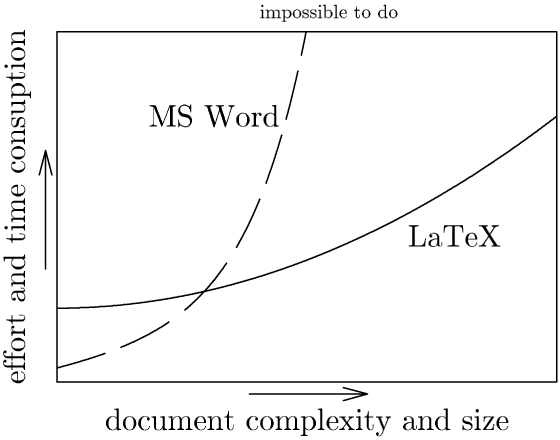
\includegraphics[width=0.5\linewidth]{Figures/latex-vs-word.png}
    \caption{Comparaison de Word et \LaTeX : effort et temps consommés en fonction de la complexité et taille du document. Source : Marko Pinteric}
    \label{fig:latex-vs-word}
\end{figure}

Je pense que pour débuter, un outil comme Overleaf est idéal. Il s'agit d'une plateforme en ligne de création de documents \LaTeX , dont la version gratuite est largement suffisante.
Cela permet de s'affranchir de l'installation d'un outil dédié et, plus particulièrement, de sa configuration (installation de packages...). Overleaf fournit d'emblée l'ensemble des librairies couramment utilisées.
On crée un compte et l'on peut directement commencer à écrire : le résultat s'affiche après quelques secondes en parallèle à l'écran.

\begin{figure}[]
    \centering
    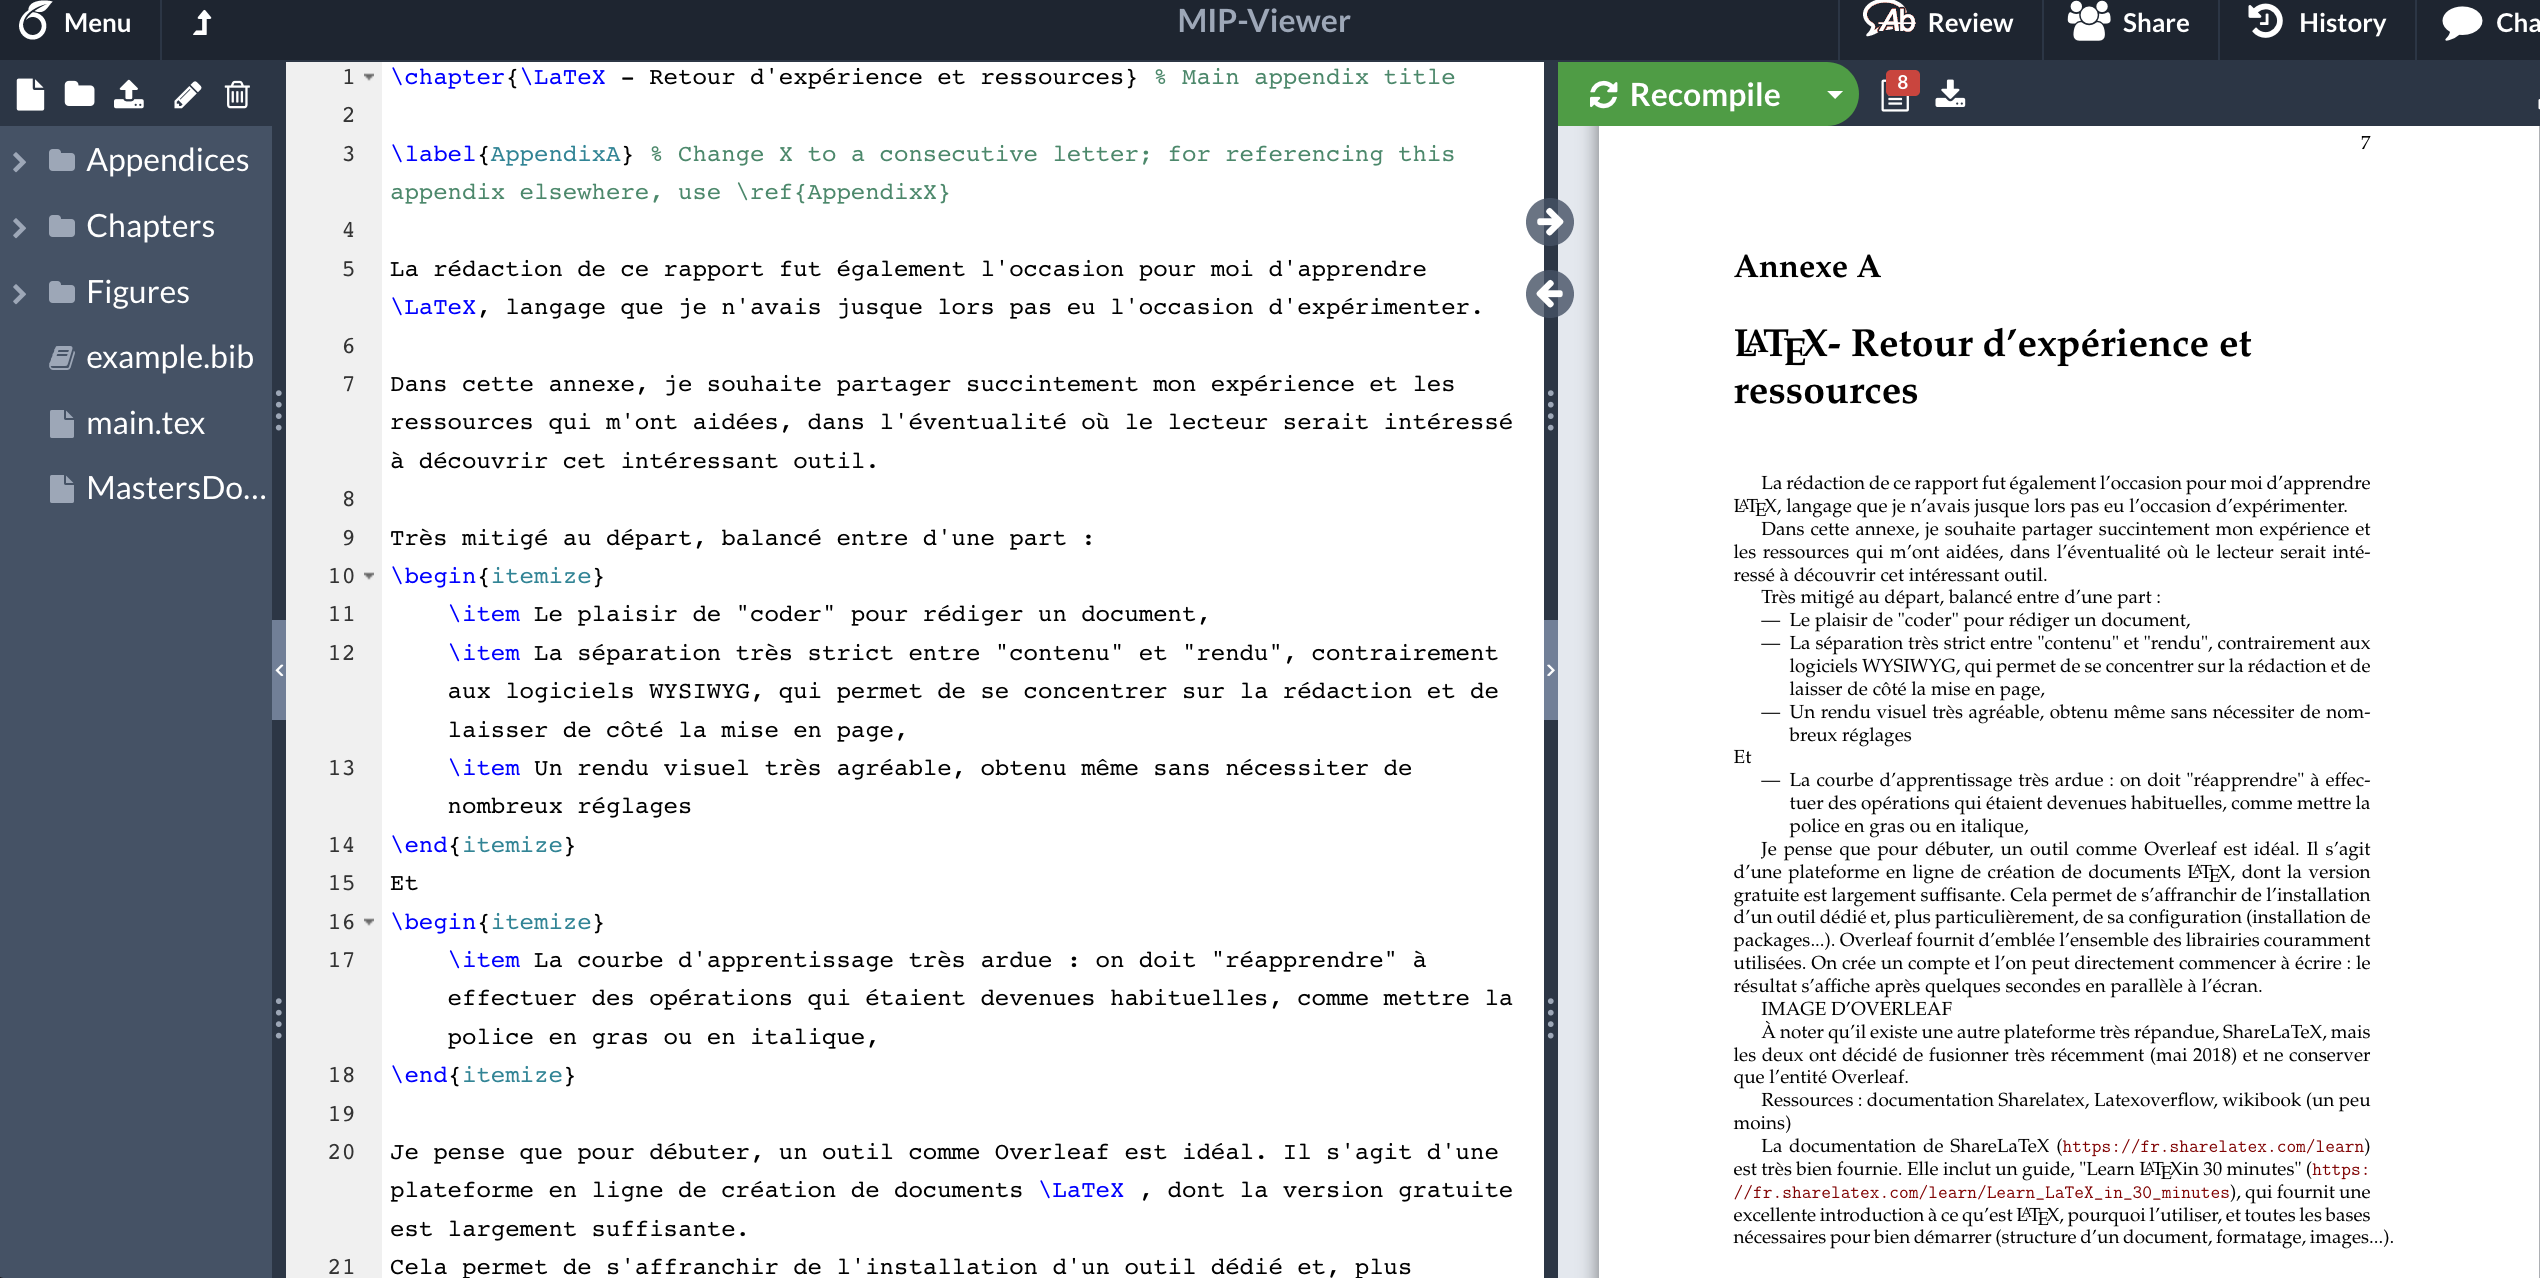
\includegraphics[width=\linewidth]{Figures/overleaf-editor.png}
    \caption{Éditeur d'Overleaf, avec le rendu à droite}
    \label{fig:overleaf-editor}
\end{figure}

À noter qu'il existe une autre plateforme très répandue, ShareLaTeX, mais les deux ont décidé de fusionner très récemment (mai 2018) et ne conserver que l'entité Overleaf.


Ressources : documentation Sharelatex, Latexoverflow, wikibook (un peu moins)

La documentation de ShareLaTeX (\url{https://fr.sharelatex.com/learn}) est très bien fournie. Elle inclut un guide, "Learn \LaTeX in 30 minutes" (\url{https://fr.sharelatex.com/learn/Learn_LaTeX_in_30_minutes}), qui fournit une excellente introduction à ce qu'est \LaTeX, pourquoi l'utiliser, et toutes les bases nécessaires pour bien démarrer (structure d'un document, formatage, images...).